\documentclass[12pt,a4paper,parskip]{scrreprt}
\usepackage[english,german,ngerman]{babel}
\usepackage[utf8]{inputenc}
\usepackage[T1]{fontenc}
\usepackage{amsmath}
\usepackage{amsfonts}
\usepackage{amssymb}
%http://www.namsu.de/Extra/pakete/Setspace.html
\usepackage{setspace}
\usepackage{makeidx}
\makeindex
\usepackage{graphicx}
%Für Quellcodeschnippsel
%Anleitung: https://en.wikibooks.org/wiki/LaTeX/Source_Code_Listings
\usepackage{listings}
\usepackage{color}

\definecolor{mygreen}{rgb}{0,0.6,0}
\definecolor{mygray}{rgb}{0.5,0.5,0.5}
\definecolor{mymauve}{rgb}{0.58,0,0.82}

\lstset{ %
  backgroundcolor=\color{white},   % choose the background color; you must add \usepackage{color} or \usepackage{xcolor}
  basicstyle=\footnotesize,        % the size of the fonts that are used for the code
  breakatwhitespace=false,         % sets if automatic breaks should only happen at whitespace
  breaklines=true,                 % sets automatic line breaking
  captionpos=b,                    % sets the caption-position to bottom
  commentstyle=\color{mygreen},    % comment style
  deletekeywords={...},            % if you want to delete keywords from the given language
  escapeinside={\%*}{*)},          % if you want to add LaTeX within your code
  extendedchars=true,              % lets you use non-ASCII characters; for 8-bits encodings only, does not work with UTF-8
  frame=single,	                   % adds a frame around the code
  keepspaces=true,                 % keeps spaces in text, useful for keeping indentation of code (possibly needs columns=flexible)
  keywordstyle=\color{blue},       % keyword style
  language=Octave,                 % the language of the code
  otherkeywords={*,...},           % if you want to add more keywords to the set
  numbers=left,                    % where to put the line-numbers; possible values are (none, left, right)
  numbersep=5pt,                   % how far the line-numbers are from the code
  numberstyle=\tiny\color{mygray}, % the style that is used for the line-numbers
  rulecolor=\color{black},         % if not set, the frame-color may be changed on line-breaks within not-black text (e.g. comments (green here))
  showspaces=false,                % show spaces everywhere adding particular underscores; it overrides 'showstringspaces'
  showstringspaces=false,          % underline spaces within strings only
  showtabs=false,                  % show tabs within strings adding particular underscores
  stepnumber=2,                    % the step between two line-numbers. If it's 1, each line will be numbered
  stringstyle=\color{mymauve},     % string literal style
  tabsize=2,	                   % sets default tabsize to 2 spaces
  title=\lstname                   % show the filename of files included with \lstinputlisting; also try caption instead of title
}
%Überflüssig, dank Dokumentenklasse scrreprt
%\usepackage[left=4.00cm, right=2.00cm, top=4.00cm, bottom=2.00cm]{geometry}
%Glossar anschalten und in TOC aufnehmen und erzeugen
%https://en.wikibooks.org/wiki/LaTeX/Glossary
\usepackage{hyperref} %Klickbare Einträge im Glossar
%\usepackage[toc,acronym]{glossaries}
%\makeglossaries
%\usepackage[nomain,acronym,xindy,toc]{glossaries} % nomain, if you define glossaries in a file, and you use \include{INP-00-glossary}
%http://tex.stackexchange.com/questions/111192/problems-with-xindy-and-glossaries
%\usepackage[nonumberlist,nomain,acronym,toc]{glossaries}
% Acronym muss an erster Stelle stehen, sonst funktioniert die Trennung von Abkürzungsverzeichnis und Glossar nicht
\usepackage[acronym,nonumberlist,toc]{glossaries}
%Glossareinträge
\newglossaryentry{GPLv2}
	{
 	 name=GPLv2,
 	 description={is a programmable machine that receives input,
               stores and manipulates data, and provides
               output in a useful format}
	}
\newglossaryentry{psu}
	{
	name=PSU,
	description={Power Supply Unit, Netzteil},
	plural=PSUs
	}
\newglossaryentry{sla}
	{
	name=SLA,
	description={Service Level Agreement}
	}
%Glossareinträge Ende
%Acronyme
\newacronym{rz}{RZ}{Rechenzentrum}
\newacronym{ram}{RAM}{Random Access Memory}
\newacronym{ca}{CA}{Computer Associates}
\newacronym{fc}{FC}{Fibre Channel}
\newacronym{elk}{ELK}{Elasticsearch - Logstash - Kibana}
\newacronym{it}{IT}{Informationstechnik}
\newacronym{omd}{OMD}{Open Monitoring Distribution}
\newacronym{os}{OS}{Betriebssystem}
\newacronym{etc}{etc.}{etcetera}
\newacronym{itil}{ITIL}{Information Technology Infrastructure Library}
\newacronym{sla}{SLA}{Service Level Agreement}
\newacronym{snmp}{SNMP}{Simple Network Management Protocol}
\newacronym{dv}{DV}{Datenverarbeitung}
\newacronym{bspw}{bspw.}{beispielsweise}
\newacronym{zb}{z.B.}{zum Beispiel}
\newacronym{nrpe}{NRPE}{Nagios Remote Plugin Executor}
\newacronym{san}{SAN}{Storage Area Network}
\newacronym{psu}{PSU}{Power Supply Unit}
\newacronym{rest}{REST}{Representational State Transfer}
\newacronym{api}{API}{Application Programming Interface}
\newacronym{cpu}{CPU}{Central Processing Unit}
\newacronym{itsm}{ITSM}{IT Service Management}
\newacronym{llc}{LLC}{Limited Liability Company}
\newacronym{obs}{OBS}{Open Build Service}
\makeglossaries
%\usepackage{imakeidx}
%Tiefe der Nummerierung ändern, Subsubsection ist Ebene 3
%\setcounter{secnumdepth}{3}
% Bibliothek & Zitierstil
\usepackage[style=authortitle-icomp,backend=biber]{biblatex}
\usepackage[babel,german=guillemets]{csquotes}
%\bibliography{seminararbeit_monitoring.bib} %U.u. deprecated
% Anleitung zu BibLaTEX: http://biblatex.dominik-wassenhoven.de/download/DTK-2_2008-biblatex-Teil1.pdf
\addbibresource{seminararbeit_monitoring.bib}
%URLs im Literaturverzeichnis in eine neue Zeile schreiben
%Quelle: http://www.golatex.de/biblatex-literaturverzeichnis-zeilenumbruch-vor-url-t8406.html
\DeclareFieldFormat{url}{\newline URL: \url{#1} }
\setuptoc{toc}{bibliography=totoc}
% Abkürzungsverzeichnis mit Nomencl
% siehe http://texwelt.de/wissen/fragen/4942/wie-kann-ich-die-erstellung-eines-abkurzungsverzeichnisses-mit-dem-paket-nomencl-automatisieren
% und http://golatex.de/abkuerzungsverzeichnis-mit-texmaker-t8301.html
% Zum aktualisieren muss "Makeindex" aufgerufen werden, Konfiguration siehe letzter Link
%\usepackage[intoc]{nomencl}
% Befehl umbenennen in abk
%\let\abk\nomenclature
% Überschrift
%\renewcommand{\nomname}{Abkürzungsverzeichnis}
% Punkte zw. Abkürzung und Erklärung
%\setlength{\nomlabelwidth}{.20\hsize}
%\renewcommand{\nomlabel}[1]{#1 \dotfill}
% Zeilenabstnde verkleinern
%\setlength{\nomitemsep}{-\parsep}
%\makenomenclature
% Ende Abkürzungsverzeichnis
\author{Markus Österle}
\title{Monitoring in Rechenzentren am Beispiel von Linux Systemen}
\date{} % setzt ein leeres Datum und löscht quasi das per default verwendete \today von der Titelseite
\begin{document}

	\maketitle
	\setcounter{tocdepth}{3}
	\tableofcontents
	% Gibt das Latex Logo aus...Stelle? 
	%\LaTeXe{}
%Ab hier 1.5facher Zeilenabstand 
	\onehalfspacing
	\chapter{Einleitung}
Das Thema des Servermonitorings hat sich im professionellen \acrshort{rz} Umfeld in den letzten Jahren zu einem großen Thema entwickelt. Durch die steigende Komplexität der Systeme steigen auch die Anforderungen an die Überwachung der selbigen, reichte es in den 90er Jahren noch aus von einem zentralen Rechner (gemeint ist hier ein normaler Personal Computer) per Ping zu Überwachen ob Rechner verfügbar sind, so wird heute ein sehr viel feineres Monitoring erwartet. Nicht nur die Erreichbarkeit der Rechner soll überwacht und statistisch aufbereitet werden, sondern auch die Auslastung und die Gesundheit einzelner Bauteile (bspw. \gls{psu}, \acrshort{ram} Bausteine). \\

In der vorliegenden Arbeit wird das Thema und die Historie des Servermonitorings unter Begrenzung auf das Teilgebiet Linux-Systeme betrachtet. Dies hat zum einen den Grund, dass der Autor viele Jahre Erfahrung mit Linux und Unix Betriebssystemen vorweisen kann und schon einige Erfahrung mit der Überwachung von *nix-Servern gemacht hat.
	\section{Warum Monitoring im Rechenzentrum?}
	
		Überwachung der Serverauslastung
		
		Proaktive Erkennung von (Hardware)Defekten
		
		\gls{sla} Überwachung
		\subsection{Warum Linux?}
		Wie in der Einleitung schon beschrieben ist die Systemüberwachung von Linux Systemen eine der am einfachsten umzusetzenden, die Ergebnisse dieser Arbeit könnten von jedem Studenten der Informatik umgesetzt und bspw. für die Überwachung privater Webservices, privater Netzwerkinfrastrukturen, SmartHomes, Wetterstationen, etc. genutzt werden. Darüberhinaus fallen bei Linux für das Betriebssystem keine Lizenzkosten.
	
	\chapter{Vom Ping zum proaktiven Monitoring}
	In den folgenden Unterkapiteln werde ich mich mit der grundlegenden Definiton von Begriffen rund um das Thema Monitoring/Serverüberwachung beschäftigen und einen kleinen Überblick über die Historie geben.
	\section{Historie}
	große Maschinen die alle Software gebündelt hatten und einfacher zu überwachen waren
	Zersplitterung der Software auf viele kleinere Maschinen, dadurch erhöhter Überwachungsaufwand, zusärtlich auch gestiegene Anforderungen an Verfügbarkeit und damit auch an eben dieses Monitoring.
	Top und seine Derivate, SAR Daten (Sysstat) die aber erst vom Server geholt und grafisch (KSar) aufbereitet werden müssen. Systemlogs die in ihrer Vielzahl unüberblickbar sind und um Sie überhaupt verarbeiten zu können auf jeden Fall gefiltert und aufbereitet werden müssen. Auch eine zunehmende Standardisierung der IT Prozesse wie beispielsweise \gls{itil}\ (\glsdesc{itil}) tragen ihren Teil zur Notwendigkeit von immer umfangreicheren Monitoring und Reportingsystemen bei.
	\subsection{ITIL die Quelle allen Übels?}
	Definition ITIL - ITIL \& Monitoring?
	Definition SLA
	Definition Servicelevel
	Was verbirgt sich nun hinter magischen Begriffen wie \gls{itil} und Monitoring, in der folge werde ich versuchen die gebräuchlichsten Definitionen darzulegen und zu beschreiben wie die einzelnen Spielarten des Monitorings mittels Tools im praktischen Teil der Arbeit umgesetzt werden.
	\section{Definition (Server-/System-)Monitoring}
	\subsection{Allgemein}
	Definition Monitoring
	\subsection{proaktives Monitoring}
	%http://www.thefreedictionary.com/proactive
	Unter \glqq proaktiv\grqq\ versteht man 
	Unter \glqq proaktivem Monitoring\grqq\ versteht man bei ITIL: \glqq Das proaktive Monitoring in seiner Überwachung achtet auf bestimmte Verhaltensmuster (Patterns), um künftige Ausfälle vorauszusehen. \grqq\ 
	Notwendig möglichst viele Informationen zu haben um Muster erkennen zu können.
	\subsection{reaktives Monitoring}
	\subsection{Verfügbarkeitsmonitoring}
	Historie
	\subsection{SLA Monitoring}
	Einhaltung vereinbarter Servicelevel \footcite[40]{iso20000sla}
	\subsection{Fazit}
	Um alle in den vergangenen Unterkapiteln beschriebenen Anforderungen zu erfüllen ist es notwendig mehrere Überwachungstechnologien zu verbinden, um ein optimales Monitoring zu erhalten. So ist es zur proaktiven Erkennung von Fehlern zum einen unerlässlich die Einträge in Logfiles auswerten zu können, um Fehler zu bemerken lange bevor Sie beginnen sich auf den Produktivbetrieb auszuwirken (bspw. Schreibfehler auf ein per \acrlong{fc} (\acrshort{fc}) angebundenes \gls{san}-System oder einfach I/O Fehler auf eine der Systemfestplatten) und zum anderen auch die Performance der Systeme im Auge zu behalten um sicher zu stellen, dass die Dimensionierung der Systeme richtig ist und nicht plötzliche Engpässe auftreten können.
	\chapter{Monitoring Systeme für Linux Server}
	Wenn man zu dem Thema \glqq Monitoringsysteme für Linux\grqq\ im Internet recherchiert wird man neben den diversen teuren Softwarelösungen diverser Hersteller immer wieder über einen Namen stolpern: Nagios. Das Tool hat sich fürs Monitoring von Linux Systemen zu einer Art Industrie Standard entwickelt. Das mag zum einen an seiner freien Verfügbarkeit liegen, zum anderen aber vielleich t auch daran, dass im Linux Umfeld viele Administratoren die Quelloffenheit und die leichte Erweiterbarkeit mittels eigener Tools, Plugins, Agenten von Nagios schätzen. \\
	
	Der Name Nagios ist wie viele Namen im Linux Umfeld ein rekursives Akronym.
	\section{Performance \& SLA Monitoring}
	\subsection{Nagios}
	\begin{figure}
	\centering
	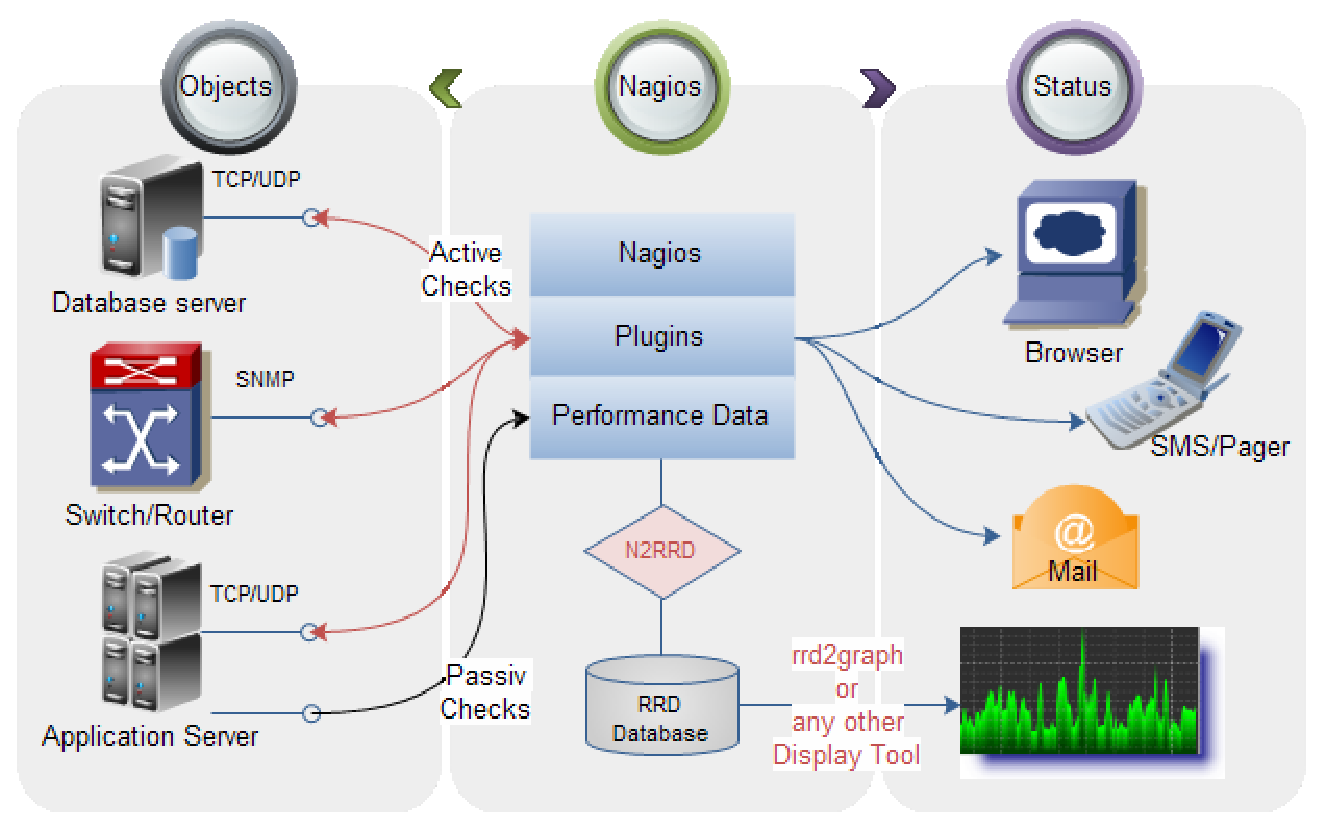
\includegraphics[scale=.5]{pics/NagiosMonitoring.eps}
    \caption[Grober Aufbau von Nagios]{Aufbau einer Nagios Appliance (Quelle: „Monitoring“ von Diglinks in der Wikipedia auf Englisch - Übertragen aus en.wikipedia nach Commons durch Esquilo.. Lizenziert unter Gemeinfrei über Wikimedia Commons - https://commons.wikimedia.org/wiki/File:Monitoring.png\#/media/File:Monitoring.png)}
	\end{figure}
	\begin{figure}
	\centering
	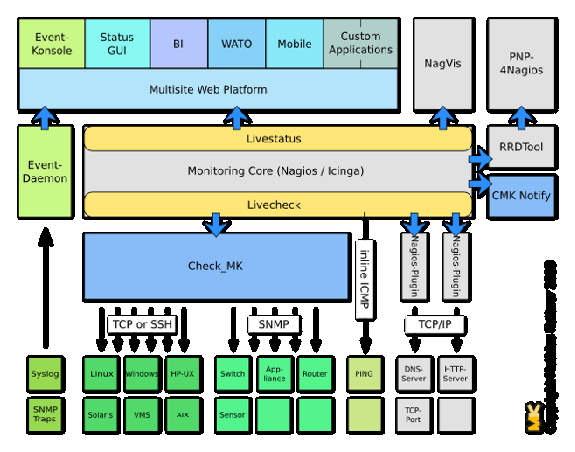
\includegraphics[]{pics/OMD_Schema.eps}
    \caption[Aufbau von Check\_MK]{Aufbau von Check\_MK (Quelle: \cite{checkmk})}
	\end{figure}
	\subsubsection{Historie}
	Nagios -> Kritik Weiterentwicklung Ethan Galstedt...siehe Lehrgangsunterlagen QSkills
	Icinga, Shinken
	check\_mk als Bundle Lösung die verschiedene Backends bereithält, inkl. mittlerweilen eigenem Backend (Microkernel)
	Fertige Lösung im Bundle mit mehr Tools
	OMD -> checkmk Änderung im Subskriptionsmodell
	check\_mk Versionen Freie Version, Subskriptionen: Innovation, Stable, etc.
	
	\subsubsection{Lizenzmodell}
	Erläuterung GPLv2
	\gls{GPLv2}
	\subsubsection{Funktionsumfang}
	\section{Logfile Monitoring}
	\subsection{Syslog-ng und Rsyslog}
	Der erste Gedanke fällt hierbei auf die in den bisherigen BS Vorlesungen gelernten Technologien, weshalb ich hier von dem Schema ein Tool aus der offenen und eines aus der kommerziellen Welt abweichen möchte.
	Problematisch in nicht homogenen Umgebungen mit verschiedenen Versionen aktueller Distributionen, weil systemd...ELK Stack ist hier besser weil vielseitiger
	\footcite{systemd2015}
	%\subsection{Splunk Monitoring}
	\subsection{Elasticsearch - Logstash - Kibana}
	Oftmals auch \acrshort{elk} oder ELK-Stack genannt sind eigentlich die drei voneinander unabhängige Tools \acrlong{elk}. 
	\chapter{Praktische Vorstellung der Funktionalität eines Monitoring Systems}
	\section{Versuchsaufbau}
	\subsection{verwendete Software}
	Opensuse Leap 42.1 als Betriebssystem für den Überwachungsrechner auf dem sowohl die Check\_MK Instanz läuft, als auch der ELK Stack. Der entfernte Rechner der per check\_by\_ssh abgefragt wird ist ein virtueller Server bei einem großen Hoster, als Betriebssystem läuft auf diesem Rechner Opensuse 13.2 (64bit) mit der für Webserver üblichen Software (LAMP-Stack = Linux Apache Mysql PHP) und zusätzliche zwei Java Anwendungen (Jenkins \& Sonarqube). An zusätzlicher überwachter Sicherheitssoftware ist Fail2Ban installiert und so konfiguriert, dass Hosts die 3 fehlerhafte Versuche sich per SSH einzuloggen unternehmen automatisch für eine bestimmte Zeit auf eine Sperrliste in der Firewall gesetzt werden. \\
	\begin{table}[h] %Quelle: http://www.weinelt.de/latex/table.html
	\begin{center}
	\begin{tabular}{|c|c|c|}
	\hline 
	eingesetzte Software & Version & Client oder Server \\ 
	\hline 
	Opensuse & 13.2 & Server\\ 
	\hline 
	Opensuse & Leap 42.1 & Client\\
	\hline
	Apache & 2.4 & Server\\
	\hline
	\end{tabular} 
	\caption[Eingesetzte Softwareversionen]{Für den praktischen Teil der Arbeit eingesetzte Softwareversionen mit ihrem Einsatzort}
	\end{center}
	\end{table}
	\subsection{Konfiguration}
	\section{Performancemonitoring}
	\subsection{Überwachung eines entfernten Servers}
	\begin{lstlisting}[language=bash]
	root@linux# ssh -i check_mk.key targethost
	\end{lstlisting} \footcite{checkmkCheckBySSH2015}
	\subsection{Überwachung einer Datenbank}
	\section{Service Level Agreement Monitoring}
	\subsection{Überwachung der Verfügbarkeit einer Datenbank}
	MySQL DB und Derby als Beispiel für die Überwachung einer in Memory Datenbank.
	\subsection{Überwachung der Verfügbarkeit einer Webseite}
	% Abkürzungsverzeichnis auf einer neuen Seite ausgeben
	%\printnomenclature
	% Literaturverzeichnis ausgeben und als Eintrag gleichwertig mit einem Kapitel ins Inhaltsverzeichnis eintragen
	\begingroup
	\nocite{*} %Alle Einträge des Literaturverzeichnisses auch ohne Zitierung ausgeben
	\printbibliography 
	\addchaptertocentry{}{Literatur}
	%\addcontentsline{toc}{chapter}{Literatur}
	\endgroup
	\printglossary[title=Abkürzungsverzeichnis, type=\acronymtype] % prints just the list of acronyms	
	\printglossary[title=Glossar]
	%\printglossaries	
	\listoffigures % Abbildungsverzeichnis
	\addchaptertocentry{}{Abbildungsverzeichnis}
	\listoftables % Verzeichnis der Tabellen
	\addchaptertocentry{}{Tabellenverzeichnis}
\end{document}